%!TEX root = ../master.tex
\chapter{Initial Problem}\label{ch:iniprob}
In this section, the basic criteria for this semester project will be explained. From this, the initial problem will be defined.

The goal of this project is to develop an 'augmented' board game that makes use of computer vision. Based on this, as well as the semester requirements, five basic criteria for the project are defined:

\begin{enumerate}
	\item The product of this project must be a media artefact.
	\item The artefact must implement computer vision in such a way that makes it interactive.
	\item The artefact must include an existing board game that we have access to.
	\item The chosen board game must not have an average game time of over two hours.
	\item The implemented computer vision must not make the act of playing more convoluted.
\end{enumerate}

The board game chosen for this project is Terra Mystica.

\section{A short introduction to Terra Mystica}
Terra Mystica is a strategy board game for 2-5 players about territory control and resource management. Each player can choose one of 14 races, each of which has their own playstyle. The board consists of hexes with different kinds of terrain. Players can only build structures on hexes with terrain which matches their race. This terrain can, however, be modified by players if they choose to spend the required resources. Finally, the game involves a Power mechanics; if a player modifies a piece of terrain next to the structures of another player, that player can choose to gain Power at the cost of Victory Points, which can be spent on acquiring resources.  

Victory Points are gained based on objectives, some of which are global (obtainable by each player), while the others are race-specific. The winner is the player that has the most Victory Points at the end of the game.

\section{An interactive board for Terra Mystica}
This project aims to create an interactive board for Terra Mystica, that uses Computer Vision to detect hand contact on the board via a camera below the surface of it. With the hand contact the user should be able to change the hexagon-shaped tiles in the game. The idea is that the board itself is a projection from below, and the board should then be changed due to inputs on the interaction with the board's surface. 

\begin{figure}[!h]
\centering	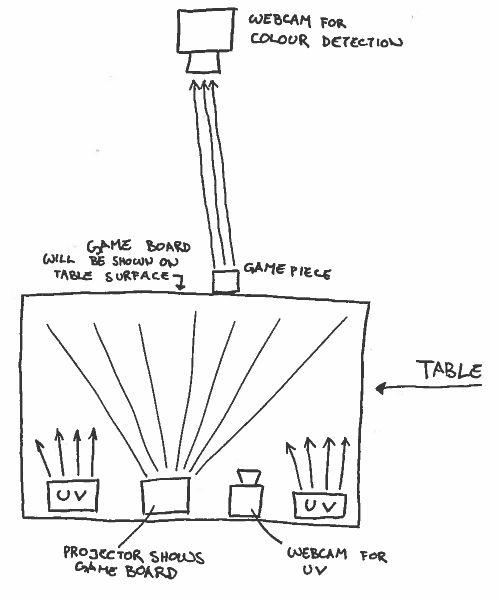
\includegraphics[width=0.5\textwidth]{TouchBoardDiagramSketch}
\end{figure}

\todo {I am uncertain if the following text has any relevance here or it should be added in the report later. }
Another feature was thought as a possible expansion of the project's product, would be board's detection of game pieces, which can be used to measure amount of 'power' after game piece placement. This would be done through computer vision detection from above, which must be able to tell difference between kinds of game pieces and ownership of them.

\section{Problem statement}
From this, an initial problem statement is defined: 

\textit{How can a media artefact that 'augments' Terra Mystica through an implementation of Computer Vision be developed?}

To answer this question, research questions are defined:

\textit{How can Computer Vision be used to facilitate user interaction?}

\textit{How can the software for a virtual board be developed?}

\subsection{Background research}
\todo{We describe Rear Infused Illumination, and add all theory we have on the things mention if RID - for example BLOBs, contrast, illumination and so on)) }
The interaction on our game board table will be based on rear diffused illumination((ref)). As shown in figure ((ref project sketch)) this means we are going to make inputs in the augmented board game via recognition of BLOBs shown in infra-red light. 
For this to work, a table plexiglas top surface on the table's needs a diffuser. Infra-red light then needs to be shined on it from beneath the surface. When the plexiglas is pressed from above the surface, 

\todo {After this, we add the competitive analysis. This with the rest of the background research and the target group a final 'problem' formulation will be made )) }


\subsection{Target Group Explained}

\section{Final Problem Formulation}\label{sec:finalprob}

